\documentclass[a4paper,11pt]{article}
\usepackage[utf8]{inputenc}
\usepackage{graphicx}
\usepackage{amsfonts}
\usepackage[normalem]{ulem}
\usepackage{hyperref}


\begin{document}

\author{
	Giuseppe André Brando Ortega.
}
\title{Control de seguridad de una puerta mediante enlaces infrarrojos y de radio frecuencia.}
\maketitle
\begin{figure}[h]
\centering
	
\includegraphics[width=0.7\linewidth]{./logo}
\end{figure}


\newpage

\section{Introducción}
El laboratorio de electrónica tiene como objetivo principal incentivar en los estudiantes el desarrollo de proyectos que puedan ser utilizados en el diario vivir. Es por ello que decidimos construir un circuito de alarma de seguridad para una vivienda común ya que la delincuencia en los tiempos más recientes ha envuelto a nuestro país en una grave crisis  que  ocupan  cada  vez  más   la  atención  de   todas   las  personas  como receptores de las consecuencias que se desprenden de ella. 
En este documento se describirá cada una de las etapas que conforman nuestro circuito con su respectivo fundamento teórico. Además se realizara un análisis matemático de los circuitos más importantes del proyecto que nos servirán para poder hacer los cálculos teóricos. 
También se incluirá graficas de las señales obtenidas en los puntos de emisión y recepción de datos, de igual forma se tomaran datos experimentales para compararlos con los datos teóricos antes obtenidos.
Finalmente encontraremos algunas imágenes que corroboren el correcto funcionamiento de nuestro proyecto, como por ejemplo los esquemáticos realizados en ISIS para la elaboración de las placas, la distribución de los elementos usados en la baquelita y fotos del circuito de alarma totalmente terminado.

\section{Resumen}
Se desea construir un circuito de seguridad para la puerta principal de una casa el cual consta de tres circuitos que son el emisor infrarrojo, el receptor infrarrojo y el transmisor de radiofrecuencia, además del receptor de radiofrecuencia y la alarma. El circuito emisor infrarrojo va colocado en un extremo de la puerta, mientras que el circuito receptor infrarrojo va colocado en el otro extremo, y el circuito del receptor de radiofrecuencia que es el que activa la alarma va colocado en cualquier lugar dentro de la casa donde pueda ser escuchada, preferiblemente puede ser en el cuarto principal del jefe de hogar. Si alguna persona intenta violentar la seguridad de la casa tratando de abrir la puerta rompiendo los seguros, esta detecta inmediatamente esa acción debido a que se corta la comunicación entre el emisor y receptor infrarrojo que va colocado detrás de la puerta. De manera práctica este circuito se puede colocar en puertas y ventanas de las casas para evitar que las mismas sean violentadas por ladrones o personas extrañas a la casa, y así mismo como  una alarma de hogar. 
El funcionamiento del circuito se basa en emitir una ráfaga de señales luminosas infrarrojas las cuales 	están en constante comunicación entre el diodo emisor y el fototransistor pero si se interfiere esta comunicación se polariza un transistor el cual hace switchear un relé que es el que polariza al circuito transmisor de radiofrecuencia el cual me manda un bit en alto a la salida del decoder que se encuentra en el circuito del receptor de radiofrecuencia, el mismo que polariza a otro transistor que me hace switchear otro relé logrando polarizar al circuito de la alarma. 

El circuito integrado es un generador/decodificador de tonos que bien cumple con las necesidades de este diseño. Tanto el fotodiodo como el fototransistor deberán estar situados con unidades de enfoque adecuadas para mejorar el alcance. Con simples reflectores de LED's se pueden obtener alcances del orden del metro. Con lentes convexas se pueden cubrir distancias de cinco metros. 
Para el circuito interruptor vía infrarrojo empleamos un fotodiodo transmisor y un fototransistor receptor, usando un multivibrador astable con el LM555 para fijar la frecuencia del tren de pulsos que va a ser la señal a transmitir. En la parte de recepción usamos un PLL como circuito enganchador de fase el cual nos servirá para sincronizar el transmisor con el receptor. Aprovechamos el funcionamiento del PLL para controlar el switcheo de un relé que activara la segunda etapa.
Para el circuito interruptor de la segunda etapa utilizamos los módulos para la comunicación de datos a través de un enlace de RF, utilizando módulos de UHF TWS-418 y RWS-418 y un par de chips para codificación y decodificación de los que se utilizan para control remoto en sistemas de seguridad, HT12E y HT12D, respectivamente. Este juego de integrados codifica y decodifica una palabra de 12 bits, compuesta por una dirección de 8 bits y una sección de datos de 4 bits. Con esta cantidad de bits se pueden comandar 256 dispositivos diferentes, enviándoles hasta 16 comandos distintos a cada uno.
El circuito de alarma está basado en otro multivibrador astable que provoca una señal de frecuencia variable en el rango audible [20Hz-20KHz] para alimentar un parlante y escuchar distintos tonos cuando esta se active.  

\begin{itemize}
	\item Utilizar los conocimientos adquiridos en las materias de electrónica vistas en la carrera.
	\item Aprender a utilizar los softwares para la simulación y creación de PCB’s para circuitos electrónicos y digitales.
	\item Diseñar un sistema de seguridad para la puerta principal de una casa utilizando enlaces infrarrojos y de radiofrecuencia.
	\item Entender y comprender el funcionamiento completo de todos los circuitos utilizados en el proyecto.
	
	
\end{itemize}








\section{TEORÍA Y ANÁLISIS MATEMÁTICOS:}

\title{SENSOR INFRARROJO}
\subsection{\underline{Diodo LED}}
Un diodo es un dispositivo electrónico provisto de dos electrodos, cátodo y ánodo, que tiene la propiedad de ser conductor en el sentido cátodo-ánodo, pero no en el inverso.

\subsection{\underline{LED (Light Emitting Diode)}}
Es un diodo capaz de emitir luz al ser polarizado en el sentido directo.Produce una luz monocromática, tiene un bajo consumo y es muy empleado como elemento de señalización en aparatos y circuitos electrónicos. El LED debe conectarse siempre respetando su polaridad, de lo contrario, no se ilumina. Dado que el LED es muy pequeño, se señalan el ánodo y el cátodo por la longitud de las patas.
	\begin{figure}[h]
	\centering
	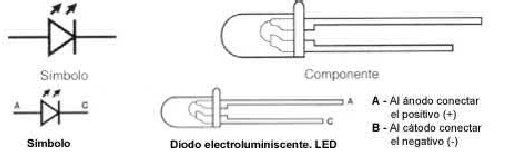
\includegraphics{./1}
	\end{figure}

La pata larga (A) corresponde al ánodo al que se conecta el polo (+) y la pata corta (C) corresponde al cátodo al que se conecta el polo (-).Los colores de las cápsulas del LED pueden ser: rojo, amarillo o verde y los diámetros más usuales son 5 y 3 mm.

\subsection{\underline{IRLED (lnfrared Light Emitting Diode)}}
Es un emisor de rayos infrarrojos que son una radiación electromagnética situada en el espectro electromagnético, en el intervalo que va desde la luz visible a las microondas. Estos diodos se diferencian de los LED por el color de la cápsula que los envuelve que es de color azul o gris. El diámetro de ésta es generalmente de 5 mm.

\subsection{\underline{Fototransistor}}
El fototransistor es un fotodetector que trabaja como un transistor clásico, pero normalmente no tiene conexión base.
	\begin{figure}[h]
	\centering
	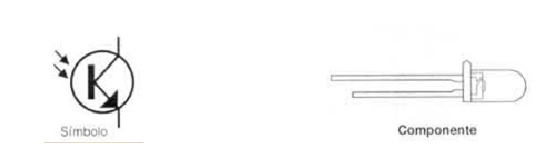
\includegraphics{./2}
	\end{figure}

En estos transistores la base está reemplazada por un cristal fotosensible que cuando recibe luz, produce una corriente y desbloquea el transistor. En el fototransistor la corriente circula sólo en un sentido y el bloqueo del transistor depende de la luz; cuanta más luz hay más conduce. El principio del fototransistor es aparentemente el mismo que el del transistor clásico. Pero si observamos el componente se ve que sólo posee dos patas, un emisor y un colector, pero le falta la base. La base de hecho es sustituida por una capa de silicio fotosensible. Si esta capa está iluminada aparece en la base una corriente que crece con la luz, lo que pone en marcha al transistor. El fototransistor reacciona con la luz visible y también con los rayos infrarrojos que son invisibles. Para distinguirlo del LED su cápsula es transparente. En el fototransistor, al igual que en los LED, la polaridad viene dada por la longitud de sus patas pero con una diferencia muy importante; en el fototransistor la pata larga es el negativo (-), al revés que en los LED, que es el positivo (+).

\subsection{\underline{Sensores reflexivos}}
Este tipo de sensor presenta una cara frontal en la que encontramos tanto al LED como al fototransistor. Debido a esta configuración el sistema tiene que medir la radiación proveniente del reflejo de la luz emitida por el LED. 
Se debe tener presente que esta configuración es sensible a la luz del ambiente que perjudicando las mediciones lo que puede dar lugar a errores. Para ello es necesario la incorporación de circuitos de filtrado en términos de longitud de onda, así pues será importante que se trabaje en ambientes de luz controlada. \\
                                                                                                                        Otro aspecto a tener en cuenta es el coeficiente de reflectividad del objeto, funcionamiento del sensor será diferente según el tipo de superficie.


\subsection{\underline{Módulos de Radio Frecuencia }}
Un enlace de radio frecuencia permite comunicarse entre dos equipos, a través de dispositivos de transmisión y recepción de datos. Para el caso del transmisor de radio frecuencia necesita el circuito integrado HT12E, y el receptor utiliza  el circuito HT12D, estos circuitos integrados asignan un código de transmisión de datos, el cual debe ser el mismo en el receptor y transmisor respectivamente, para que el sistema pueda funcionar, operan con 4 bits cada uno.  \\

\textbf{Módulo Transistor}
Tiene una potencia de salida de hasta 8 mW a 433.92 Mhz, alcanzando distancias de aproximadamente 140 metros en espacios abiertos (línea de vista) y de 60 metros en espacios internos donde se encuentran obstáculos como paredes, separadores en oficinas, etc. Este tipo de transmisor acepta señales lineales y digitales de entrada y opera con un voltaje de 1.5 V a 12 V de corriente continua.  

	\begin{figure}[h]
		\centering
		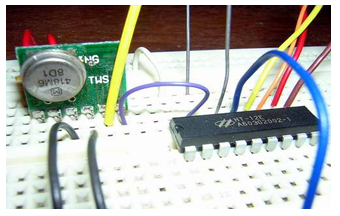
\includegraphics[width=0.7\linewidth]{./3}
	\end{figure}


\textbf{Módulo receptor}

El módulo opera a 433.92 MHz, y tiene una sensibilidad de 3 uV, opera con un  voltaje de alimentación entre 4.5V y 5.5V de corriente continua, posee una  salida lineal y una digital, además contiene un capacitor variable para el ajuste de la frecuencia de recepción.

	\begin{figure}[h]
		\centering
		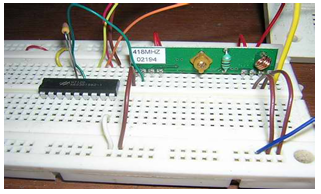
\includegraphics[width=0.7\linewidth]{./4}
	\end{figure}
	
Los elementos de un circuito para la comunicación de datos a través de un enlace de RF usados en este proyecto son los módulos de UHF TWS-418 y RWS-418, que ya se describieron antes.
En este proyecto también se utilizo dos integrados para codificación y decodificación de los que se utilizan para control remoto en sistemas de seguridad, HT12E y HT12D, respectivamente. Este juego de integrados codifica y decodifica una palabra de 12 bits, compuesta por una dirección de 8 bits y una sección de datos de 4 bits. Con esta cantidad de bits se pueden comandar 256 dispositivos diferentes, enviándoles hasta 16 comandos distintos a cada uno.
A continuación se pueden observar los circuitos utilizados.

	\begin{figure}[h]
		\centering
		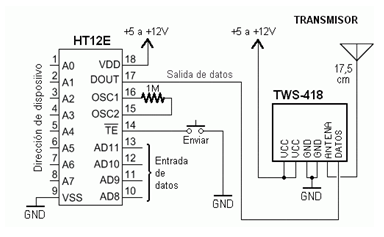
\includegraphics[width=0.7\linewidth]{./5}
	\end{figure}
	
El circuito transmisor permite el uso de una tensión de alimentación entre 5V y 12V. Esto habilita para la utilización de un amplio rango de baterías, como por ejemplo una de 9V, valor bastante típico para este uso. Las pruebas las realicé con una batería de 6V. El receptor, por las características técnicas del chip decodificador HT12D, debe funcionar exclusivamente con 5V.

	\begin{figure}[h]
		\centering
		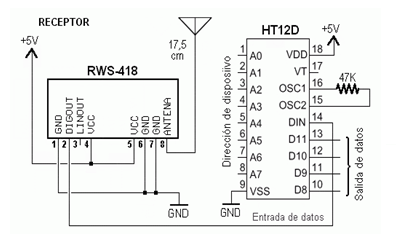
\includegraphics[width=0.7\linewidth]{./6}
	\end{figure}	
	
De antena (tanto en el receptor como en el transmisor) se recomienda utilizar un alambre de 17,5 cm. de longitud. Con esta medida el enlace funcionó muy bien, comunicándose incluso a través de paredes, aunque si se desea se pueden utilizar antenas más profesionales, claro que más costosas, obviamente. \\

La dirección de dispositivo (ingresadas a través de las patas 1 a 8 en ambos chips) no tenía importancia en esta prueba, de modo que las colocamos todas al mismo valor. La hoja de datos indica que se pueden dejar estas patas al aire (o en todo caso ponerlas todas a masa), y eso hice en las primeras pruebas: las dejé sin conexión. El enlace descripto en este trabajo funcionó con una dirección igual a \$FF ó 255. De todos modos, pruebas posteriores demostraron que es mejor poner estas patas a un nivel y no dejarlas en el aire, sea a masa o sea a un valor de +5V, porque si esto no se hace el funcionamiento puede resultar irregular. \\
	
En el integrado decodificador HT12D, la señal VT significa Valid Transmission (Transmisión Válida), es decir, cada vez que esta señal va a un nivel alto es porque el código presente en la salida de datos es un dato válido para el dispositivo receptor. No se deben usar las salidas para actuar algo directamente, se deben usar junto con esta señal VT en alto. Para cumplir esto se puede colocar una compuerta AND o un circuito similar, que cumpla la misma función de una compuerta AND (un transistor y resistores pueden servir). Con respecto a la parte de dirección, si el dispositivo HT12D no tiene la misma dirección que viene en la palabra que ha recibido, obviamente no se produce esta señal VT.	

\subsection{\underline{INTEGRADO LM555}}
Este Circuito Integrado (C.I.) es para los experimentadores y aficionados, un dispositivo barato con el cual pueden hacer muchos proyectos. Este temporizador es tan versátil que se puede utilizar para modular una señal en Amplitud Modulada (A.M.)
Está constituido por una combinación de comparadores lineales, flip-flops (biestables digitales), transistor de descarga y excitador de salida.
Las tensiones de referencia de los comparadores se establecen en 2/3 V para el primer comparador C1 y en 1/3 V para el segundo comparador C2, por medio del divisor de tensión compuesto por 3 resistores iguales R. En el gráfico se muestra el número de pin con su correspondiente función.
En estos días se fabrica una versión CMOS del 555 original, como el Motorola MC1455, que es muy popular. Pero la versión original de los 555 sigue produciéndose con mejoras y algunas variaciones a sus circuitos internos. El 555 está compuesto por 23 transistores, 2 diodos, y 16 resistores encapsulados en silicio. Hay un circuito integrado que se compone de dos temporizadores en una misma unidad, el 556, de 14 pines y el poco conocido 558 que integra cuatro 555 y tiene 16 pines.
Hoy en día, si ha visto algún circuito comercial moderno, no se sorprenda si se encuentra un circuito integrado 555 trabajando en él. Es muy popular para hacer osciladores que sirven como reloj (base de tiempo) para el resto del circuito.

\subsection{\underline{Funcionamiento del Circuito Integrado 555}}
El temporizador 555 se puede conectar para que funcione de diferentes maneras, entre los más importantes están: como multivibrador astable y como multivibrador monoestable. Puede también configurarse para por ejemplo generar formas de onda tipo Rampa.

\subsection{Multivibrador Estable}
Este tipo de funcionamiento se caracteriza por una salida con forma de onda cuadrada (o rectangular) continua de ancho predefinido por el diseñador del circuito. El esquema de conexión es el que se muestra. La señal de salida tiene un nivel alto por un tiempo t1 y un nivel bajo por un tiempo t2. La duración de estos tiempos dependen de los valores de R1, R2 y C, según las fórmulas siguientes:

	\begin{figure}[h]
		\centering
		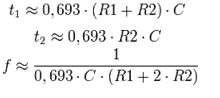
\includegraphics[width=0.7\linewidth]{./7a}
	\end{figure}

El período es simplemente $T = \frac{1}{f}$

	\begin{figure}[h]
		\centering
		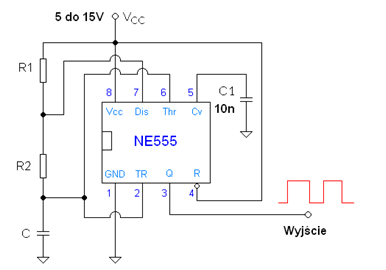
\includegraphics[width=0.7\linewidth]{./7}
	\end{figure}

\subsection{\underline{Multivibrador monoestable}}
En este caso el circuito entrega a su salida un solo pulso de un ancho establecido por el diseñador.
El esquema de conexión es el que se muestra. La fórmula para calcular el tiempo de duración (tiempo en el que la salida está en nivel alto) es:

$T = ln(3)\cdot R \cdot C$ \\ 
$T \approx 1,1 \cdot R \cdot C$

	\begin{figure}[h]
		\centering
		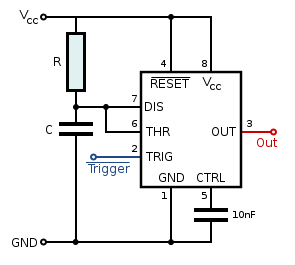
\includegraphics[width=0.7\linewidth]{./8}
	\end{figure}
	
Nótese que es necesario que la señal de disparo, en la terminal 2 del 555, sea de nivel bajo y de muy corta duración para iniciar la señal de salida.

\subsection{\underline{INTEGRADO NE567 PLL}}
Descripción:
El NE567 es un detector de tono y frecuencia integrado y también puede usarse como generador de señal cuadrada. Por medio de componentes externos puede determinarse la frecuencia central de detección, el ancho de banda de esta, el delay de la señal de salida entre otras. \\

Funcionamiento:
El integrado NE567 activara su salida a nivel bajo cuando en su entrada se detecte una señal de tono o frecuencia igual al configurado en el NE567. Para configurar estos parámetros usaremos las siguientes fórmulas:

	\begin{figure}[h]
		\centering
		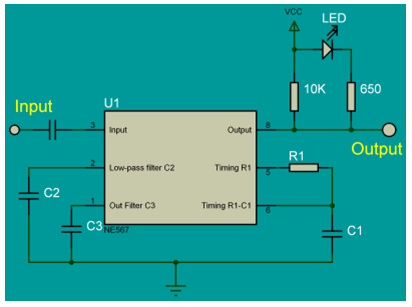
\includegraphics[width=0.7\linewidth]{./9}
	\end{figure}
	
Frecuencia central de detección: $f_0 = \frac{1}{1.1 X R1 X C1}$

Para una mejor estabilidad térmica se aconseja un valor para R1 entre 2K y 20K tal como indica en el datasheet.

Ancho de banda: $$BW	= 1070 \sqrt{\frac{V_i}{f_0 x C2}}en \% de f_0 $$

$V_i$ = Input voltage ($\leq$ 200mVRMS) 
$C_2$ = Low-pass filter capacitor ($\mu$F)

El valor del condensador C3 no es crítico y normalmente se usará la formula  $C3 = 2xC2$. Lo que hace este condensador es retardar la señal o pulso de salida, para detectar señales muy cortas se tendrá que baja su valor pero esto también hará que se active solo y sea inestable.
Mirar el datasheet para ver las curvas características del integrado e información más detallada. \\

Usos
El NE567 puede ser usado como detector de balizas para Infrarrojos con lo que podremos localizar una baliza que emita a determinada frecuencia, también puede ser usado para detección de ultrasonidos.

\newpage
\section{DIAGRAMA ESQUEMATICO DE LOS CIRCUITOS UTILIZADOS:}

	\begin{figure}[h]
		\caption{CIRCUITO EMISOR INFRARROJO}
		\centering
		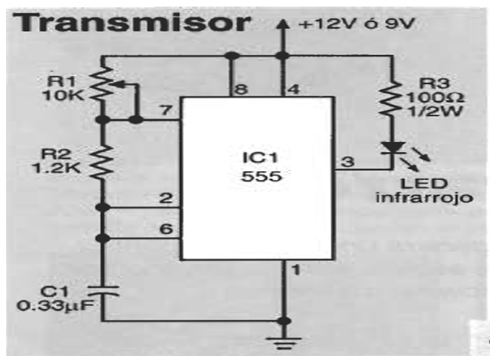
\includegraphics[width=0.5\linewidth]{./10}
	\end{figure}

	\begin{figure}[h]
		\caption{ISIS DEL CIRCUITO EMISOR INFRARROJO}
		\centering
		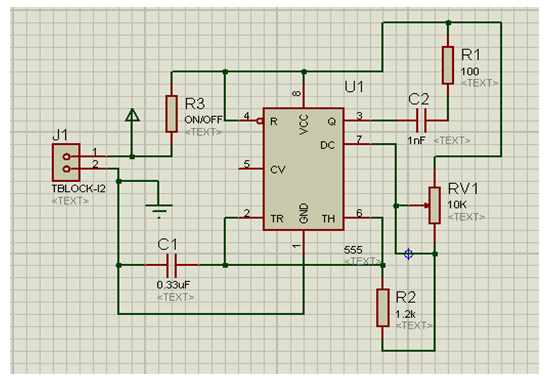
\includegraphics[width=0.6\linewidth]{./11}
	\end{figure}

	\begin{figure}[h]
		\caption{CIRCUITO RECEPTOR INFRARROJO – TRANSMISOR RF}
		\centering
		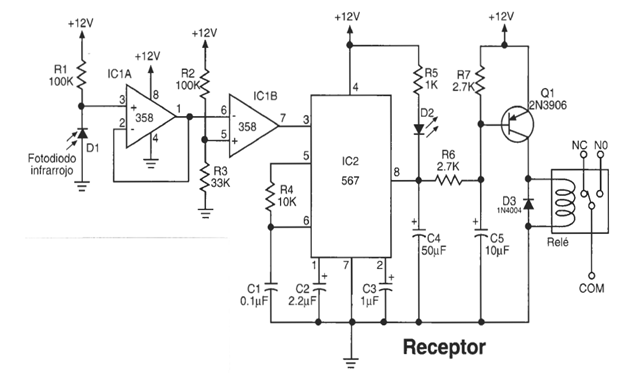
\includegraphics[width=0.6\linewidth]{./12}
	\end{figure}
	
	\begin{figure}[h]
		\caption{CIRCUITO TRANSMISOR RF}
		\centering
		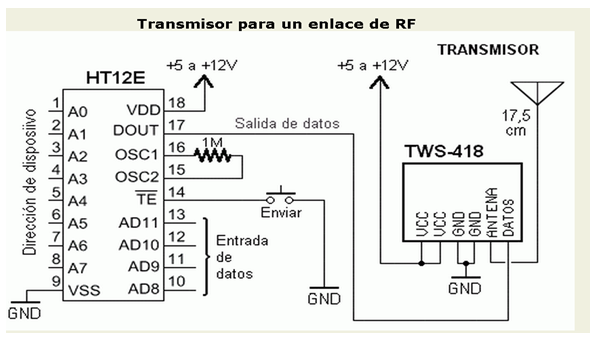
\includegraphics[width=0.6\linewidth]{./13}
	\end{figure}	
	\newpage
	\begin{figure}[h]
		\caption{ISIS DEL CIRCUITO RECEPTOR INFRARROJO – TRANSMISOR RF}
		\centering
		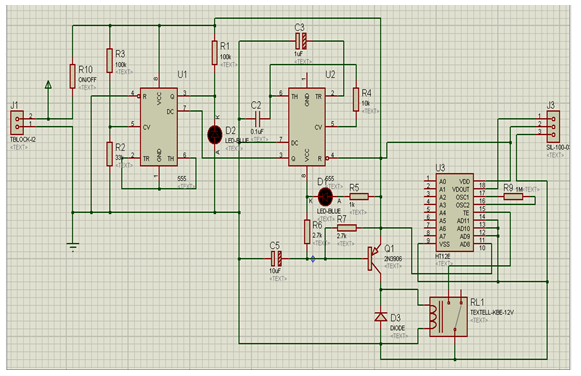
\includegraphics[width=0.6\linewidth]{./14}
	\end{figure}
%
	\begin{figure}[h]
		\caption{CIRCUITO RECEPTOR RF }
		\centering
		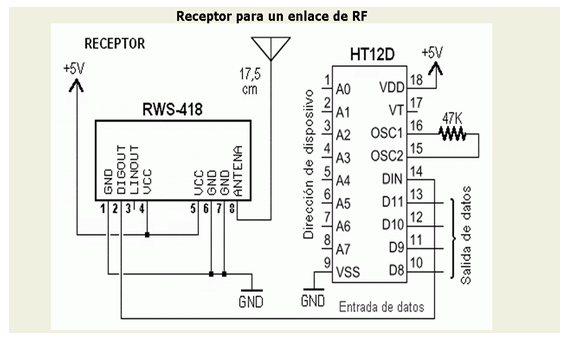
\includegraphics[width=0.6\linewidth]{./15}
	\end{figure}
%
	\begin{figure}[h]
		\caption{CIRCUITO DE LA ALARMA}
		\centering
		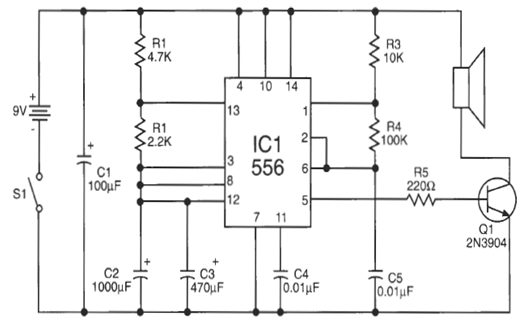
\includegraphics[width=0.6\linewidth]{./16}
	\end{figure}
%
	\begin{figure}[h]
		\caption{ISIS DEL CIRCUITO RECEPTOR RF - ALARMA}
		\centering
		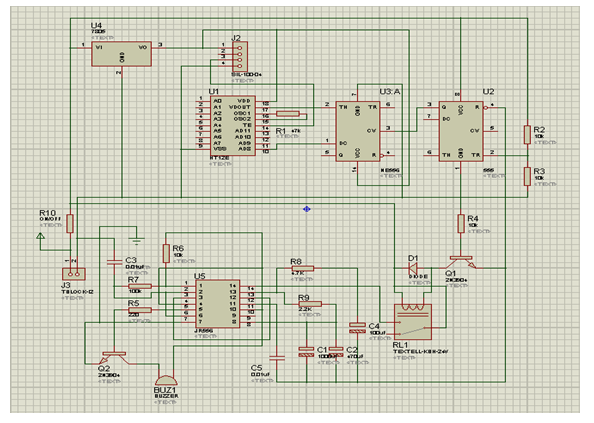
\includegraphics[width=1\linewidth]{./17}
	\end{figure}
\newpage
	\begin{figure}[h]
		\centering
		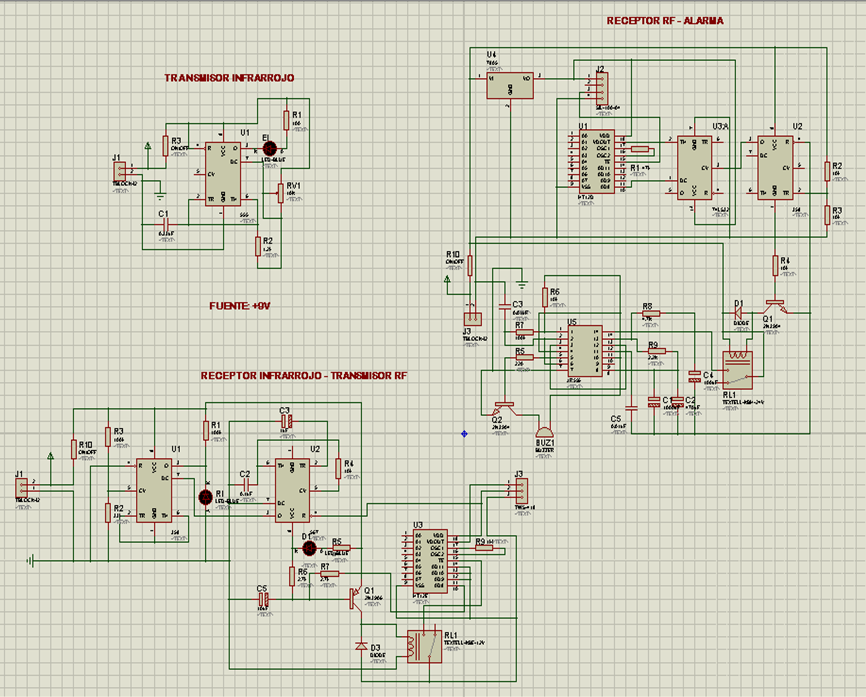
\includegraphics[width=0.9\linewidth]{./18}
	\end{figure}
\newpage

\end{document}